\documentclass[10pt]{exam}
\usepackage[T1]{fontenc}
\usepackage[paper=a4paper,margin=2cm]{geometry}
\usepackage[sfdefault,light]{roboto}

\usepackage[usenames,dvipsnames]{xcolor}
\usepackage{amsmath,amssymb,array,graphicx,enumitem,listings,lstautogobble,multicol,textcomp,titlesec}
\usepackage{mathtools}

\setlength\parindent{0cm}

%Title & Section Formatting
\titleformat{\section}{\normalfont\Large\bfseries}{}{0em}{}[{\titlerule[0.5pt]}]
\titleformat{\subsection}{\normalfont\large\bfseries}{}{0em}{}

%Mathematical Shortcuts
\newcommand{\floor}[1]{\left\lfloor #1 \right\rfloor}
\newcommand{\ceil}[1]{\left\lceil #1 \right\rceil}

%Listings Shortcuts & Settings
\newcommand{\code}[1]{\lstinline{#1}}
\lstset{language=Java,
        autogobble=true,
        basicstyle=\ttfamily,
        commentstyle=\color{black!45},
        keywordstyle=\bfseries,
        showstringspaces=false,
        upquote=true}

%General Shortcuts
\newcommand{\blankpage}{\null\thispagestyle{empty}\addtocounter{page}{-1}\newpage}

\usepackage{draftwatermark,transparent}
\SetWatermarkAngle{0}
\SetWatermarkText{\transparent{0.025}\includegraphics[scale=0.75]{graphics/logo_black.png}}

%Color-Coded questions
\newcommand{\ColourQuestion}[3]{\renewcommand{\questionlabel}{\colorbox{#1}{\bfseries\color{white}\thequestion}\hfill}\question[#3] #2}
\newcommand{\BlueQuestion}[1]{\ColourQuestion{RoyalBlue}{#1}{1}}
\newcommand{\GreenQuestion}[1]{\ColourQuestion{ForestGreen}{#1}{2}}
\newcommand{\YellowQuestion}[1]{\ColourQuestion{Goldenrod}{#1}{4}}
\newcommand{\RedQuestion}[1]{\ColourQuestion{BrickRed}{#1}{6}}
\newcommand{\PurpleQuestion}[1]{\ColourQuestion{RoyalPurple}{#1}{30}}
\pointsinrightmargin

\header{\footnotesize\scshape Assignment \#\AssignmentNumber: \AssignmentTitle}{}{}
\cfoot{\footnotesize\scshape \AssignmentCourse\\Woodstock School---Mussoorie, Uttarakhand---India}


\def\AssignmentCourse{AP Computer Science Principles}
\def\AssignmentNumber{05}
\def\AssignmentTitle{Looping}

\begin{document}
  \begin{questions}
    %While -> For loop
    \BlueQuestion{Write the following code fragment as a \code{for} loop.}
      \begin{lstlisting}
        int i = 0;
        while (i < 10) {
          ellipse(i, i, i, i);
          i++;
        }
      \end{lstlisting}

    %For -> While loop
    \BlueQuestion{Write the following code fragment as a \code{while} loop.}
      \begin{lstlisting}
        for (int i = 0; i < width; i = i + 5)
          line(i, 0, i, height);
      \end{lstlisting}

    %Syntax Errors
    \GreenQuestion{A common error beginning programmers face with the \code{for}-loop is illustrated in the code segment below:}
      \begin{lstlisting}
        for (int i = 0; i < 100; i = i + 5); 
          line(i, 0, i, height);
      \end{lstlisting}
      \begin{parts}
        \part Identify the error in the code above.
        \part This type of error is actually a \emph{semantic} error. That is, Processing accepts the code as valid; however, it will not do what appears to be intended by the programmer. What happens when the above code fragment is run and why?
      \end{parts}

    %Grid of Bees!
    \GreenQuestion{Use nested loops to create a grid of Processing Bees based on your work on the Processing Bee program from Assignment \#3.}\\
      {\small\textbf{Note:} Your program should include as many bees as possible based on the \code{width} and \code{height} of the drawing canvas. You may include some padding between consecutive bees for aesthetic reasons if you wish.}

    %Redesign Dartboard
    \YellowQuestion{Redesign your \code{Dartboard} program from Assignment \#3 to use loops wherever possible in order to drastically reduce the number of individual lines of code.}

    %Graphing a particular mathematical function?
    %Setting up a graphing window
    %Translate function?
    \RedQuestion{Although the Processing drawing canvas has a pixel coordinate statement wherein the top-left coordinate is always \code{(0, 0)} and the bottom-right coordinate is always \code{(width, height)}, it is often important to offer different ``views'' of data, requiring a transformation of the coordinate system. Implement a program that will store values for \code{xMin}, \code{xMax}, \code{xStep}, \code{yMin}, \code{yMax}, and \code{yStep} and produces a coordinate grid, including coordinate axis. This will allow us to produce a ``window'' system similar to many popular graphing calculators. See below for a number of examples.}

      \begin{minipage}{0.33\textwidth}
        \begin{center}
          \small
          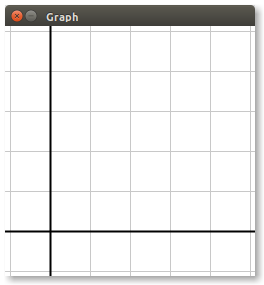
\includegraphics[scale=0.5]{files/Example1}

          \begin{tabular}{l c l c}
            \code{xMin} & -5 & \code{yMin} & -5\\
            \code{xMax} & 25 & \code{yMax} & 25\\
            \code{xStep} & 5 & \code{yStep} & 5\\
          \end{tabular}
        \end{center}
      \end{minipage}
      \begin{minipage}{0.33\textwidth}
        \begin{center}
          \small      
          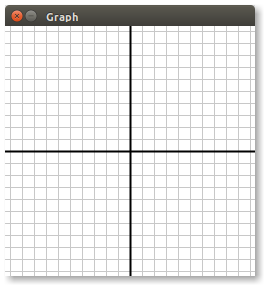
\includegraphics[scale=0.5]{files/Example2}

          \begin{tabular}{l c l c}
            \code{xMin} & -10 & \code{yMin} & -10\\
            \code{xMax} & 10 & \code{yMax} & 10\\
            \code{xStep} & 1 & \code{yStep} & 1\\
          \end{tabular}
        \end{center}    
      \end{minipage}
      \begin{minipage}{0.33\textwidth}
        \begin{center}
          \small      
          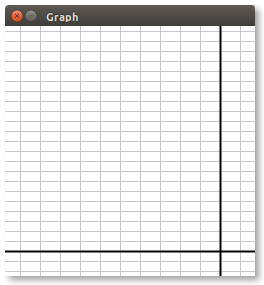
\includegraphics[scale=0.5]{files/Example3}

          \begin{tabular}{l c l c}
            \code{xMin} & -100 & \code{yMin} & 0\\
            \code{xMax} & 10 & \code{yMax} & 100\\
            \code{xStep} & 10 & \code{yStep} & 5\\
          \end{tabular}
        \end{center}            
      \end{minipage}
  \end{questions}
\end{document}
